\documentclass[Main]{subfiles}
\begin{document}

\setcounter{chapter}{2}
\chapter{System-wide design decisions}

\begin{figure}[H]
\centering
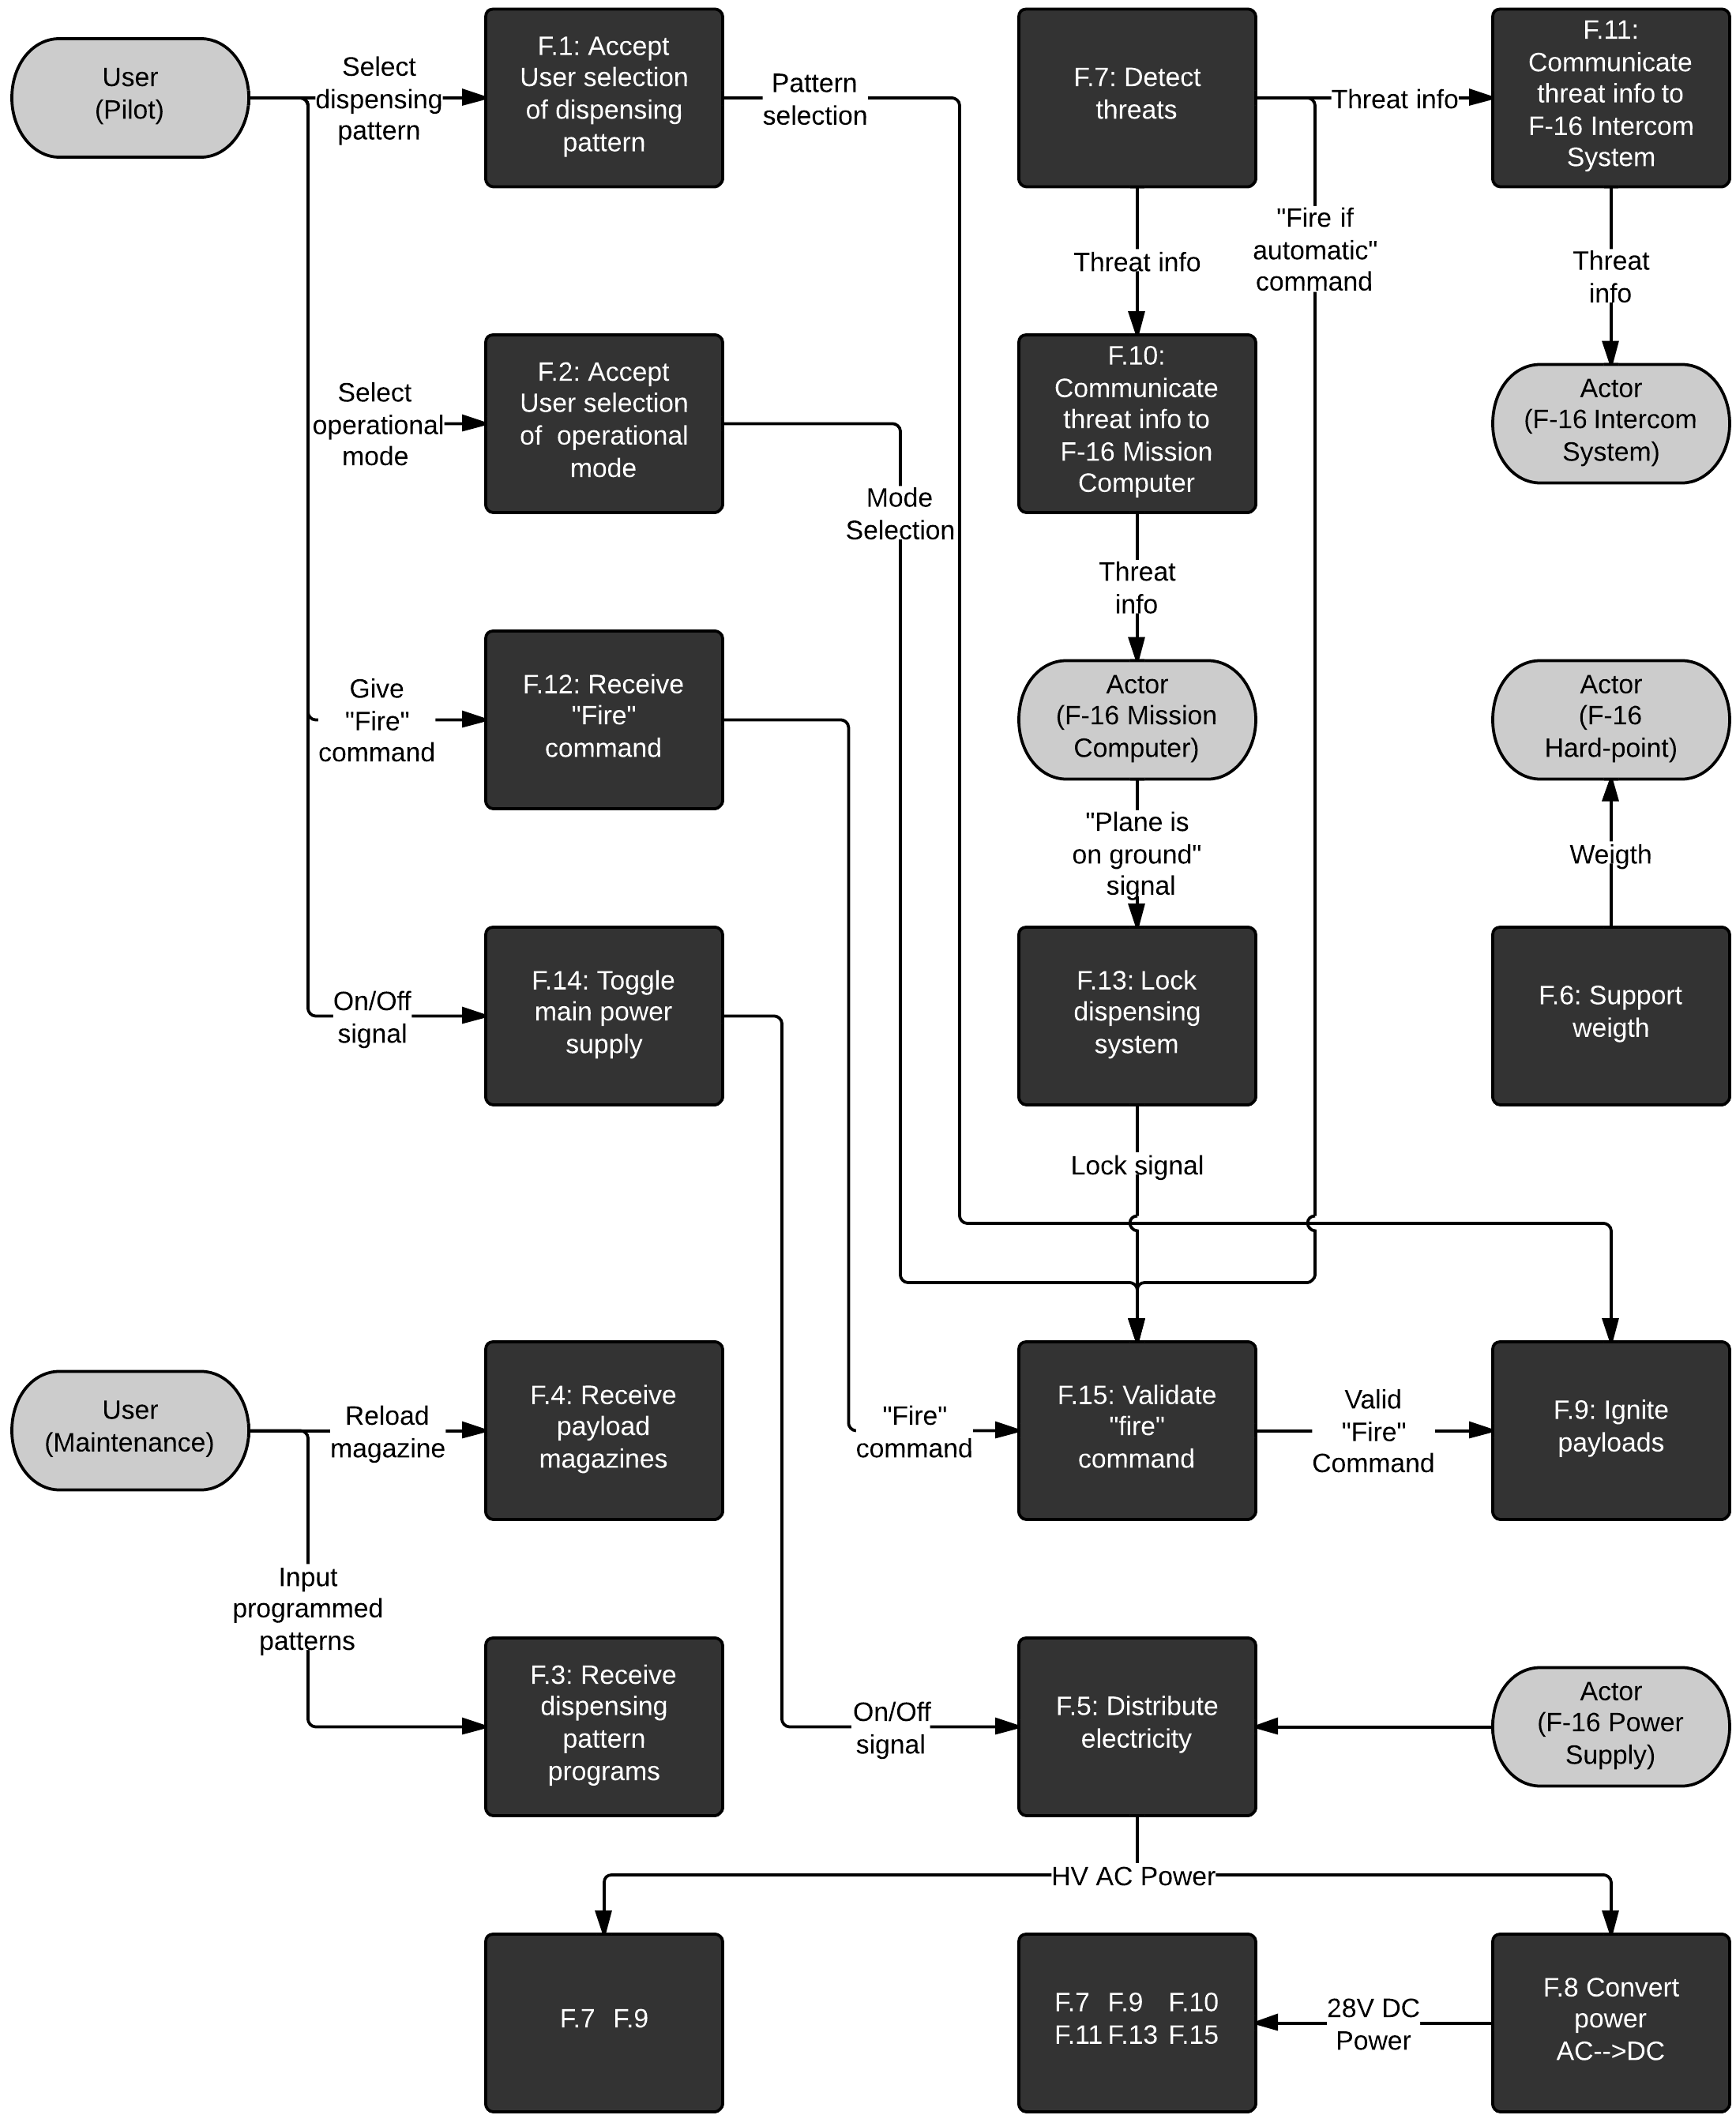
\includegraphics[width=0.97\textwidth]{FunctionalFlowDiagram}
\caption{Functional diagram}
\end{figure}


\section{Inputs and outputs}
%Design decisions regarding inputs the system will accept and outputs it will produce.

\begin{enumerate}[label=\bfseries DDD-\arabic*:]

\item The mission computer shows which mode the system is in.

\item The mission warning system provides a signal with a threat's location to the intercom system.

\item The mission computer shows how many flairs are left.

\item The mission computer shows if all DSSs are available. (SR-10)

\item The pilot can select mode with a physical unit -- either a button, flip switch or turn switch.

\item The pilot can select to fire flares of the selected pattern with a click of a button.

\item The maintenance crew can load flares form the 8 hatches in the pod.

\item The pilot can turn off the power to the pod by clicking a button, flicking a switch or turning a switch.

\end{enumerate}

\section{System behavior and performance characteristics}
%Design decisions on system behavior in response to each input or condition, including actions the system will perform, response times and other performance characteristics.

\begin{enumerate}[resume*]

\item If no more flairs are available, the system will play a sound when the fire-action would be performed.

\item The time it takes for the new mode to appear from the pilot selects a new mode shall be less than 30 ms.

\item When flairs are fires the remaining numbers shall be updated in less than 30 ms.

\item If the pilot turns on the pod after it has been disabled, the pod shall be ready in under 500 ms.

\end{enumerate}

\section{Data appearance}
%Design decisions on how system databases/data files will appear to the user.

\begin{enumerate}[resume*]

\item The angle of a threat shall be send to the cockpit unit for processing in the pilots helmet.

\item The selected mode shall be shown as text in the cockpit unit.

\end{enumerate}

\section{Safety and security measures}
%Selected approach to meet safety, security, and privacy requirements

\begin{enumerate}[resume*]

\item 

\end{enumerate}

\section{Physical appearance}
%Design and construction choices for hardware or hardware-software systems, such as physical size, color, shape, weight, materials, and markings
\begin{enumerate}[resume*]

\item The pod shall be mounted on the aircraft's left wing with standard T-hooks spaced by 13 inches.(SR-28)

\item The pod must be no longer than 120 cm, no wider than 40 cm, no taller 40 cm and aerodynamic. (RFPS, SR-3.1)

\item The pod shall be colored in FS 26373 \footnote{\url{http://www.cybermodeler.com/aircraft/f-16/vipercolors.shtml}}

\item The pod shall only have marking of font size 60 pt Impact in black (\#000000)

\end{enumerate}


\section{Other}
%Other system-wide design decisions made in response to requirements, such as selected approach to providing required  exibility, availability, and maintainability

\begin{enumerate}[resume*]

\item The flairs shall be loaded from 8 hatches in the pod by a mechanic.

\end{enumerate}

\end{document}